\chapter{ANALISIS DAN PERANCANGAN SISTEM}
\tab Pada bab ini akan dijelaskan mengenai desain dan implementasi rancangan sistem informasi untuk memantau pencapaian \textit{revenue} oleh Telkomsel Regional Jawa Timur. Sistem informasi untuk memantau pencapaian \textit{revenue} ini digunakan untuk memudahkan proses pengolahan data serta penyebaran informasi. Aplikasi web ini dikhususkan untuk internal Telkomsel.

\section{Mengelola Data \textit{Revenue}}
Berikut adalah deskripsi sistem dan diagram aktivitas pada \textit{use case} Mengelola Data \textit{Revenue}. 
\subsection{Deskripsi Umum Sistem}
\tab Sistem akan menyimpan informasi mengenai data \textit{revenue}. Data yang dimasukkan akan disimpan ke dalam basis data. Pada kegiatan ini, terdapat sebuah parameter berupa cluster mana yang akan dimasukkan datanya ke basis data.
\subsection{\textit{Use Case} dan Fitur Sistem}
Gambar \ref{figure:use_case_mengelola_data_revenue} adalah \textit{use case} mengelola data \textit{revenue}. Pada pengelolaan data \textit{revenue}, pengguna dapat melakukan beberapa kegiatan sebagai berikut:

	\begin{figure}[h]
		\centerline {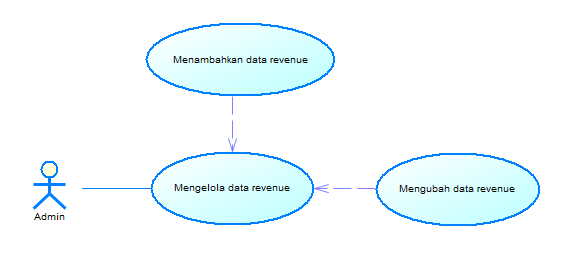
\includegraphics[width=8cm,height=4.5cm]{bab4/use_case_mengelola_data_revenue.png}}
		\caption{Diagram \textit{Use Case} Mengelola Data \textit{Revenue}}
		\label{figure:use_case_mengelola_data_revenue}
	\end{figure}
	
	\subsubsection{Menambah Data \textit{Revenue}}
	Pengguna dapat menambahkan data \textit{revenue}. Diagram \ref{figure:activity_menambah_data_revenue} adalah diagram aktivitas menambah data \textit{revenue} pada sistem TPORT. Pada pengisian form untuk mengupload data \textit{revenue}, pengguna harus menentukan rentang waktu data yang tersedia serta \textit{cluster} mana yang akan diupload datanya.
	
	\begin{figure}[h]
	\centerline {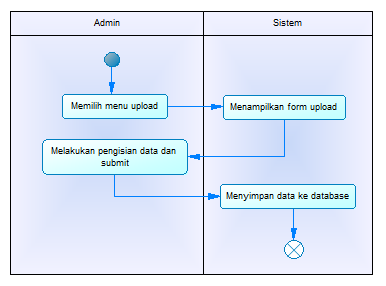
\includegraphics[width=9cm,height=6cm]{bab4/activity_menambah_data_revenue.png}}
	\caption{Diagram Aktivitas Menambah Data \textit{Revenue}}
	\label{figure:activity_menambah_data_revenue}
	\end{figure}
		
	\subsubsection{Mengubah Data \textit{Revenue}}
	Pengguna dapat mengubah data \textit{revenue}. Diagram \ref{figure:activity_mengubah_data_revenue} adalah diagram aktivitas mengubah data \textit{revenue} pada sistem TPORT. Untuk mengubah data yang sudah diupload, pengguna harus melakukan \textit{step} yang sama seperti menambahkan data baru. Sistem akan secara otomatis menggantikan data lama dengan data yang baru.
	
	\begin{figure}[h]
	\centerline {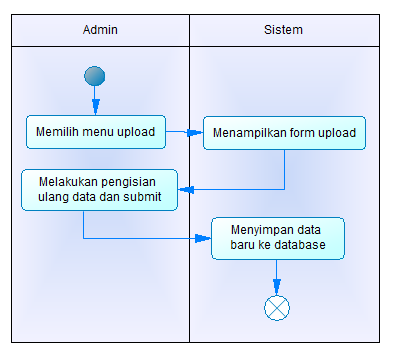
\includegraphics[width=7cm,height=5cm]{bab4/activity_mengubah_data_revenue.png}}
	\caption{Diagram Aktivitas Mengubah Data \textit{Revenue}}
	\label{figure:activity_mengubah_data_revenue}
	\end{figure}

\section{Mengelola Target Pencapaian \textit{Revenue}}
Berikut adalah deskripsi dan diagram aktivitas pada \textit{use case} Mengelola Target Pencapaian \textit{Revenue}.
\subsection{Deskripsi Umum Sistem}
\tab Sistem ini akan melakukan pengelolaan target pencapaian \textit{revenue}. Pada kegiatan ini, terdapat sebuah parameter berupa cluster mana yang akan ditentukan targetnya. Data yang dimasukkan akan disimpan ke dalam basis data.
\subsection{\textit{Use Case} dan Fitur Sistem}
Gambar \ref{figure:use_case_mengelola_target_pencapaian} adalah \textit{use case} mengelola target pencapaian \textit{revenue}. Pada pengelolaan target pencapaian \textit{revenue}, pengguna dapat melakukan beberapa kegiatan sebagai berikut:

	\begin{figure}[h]
		\centerline {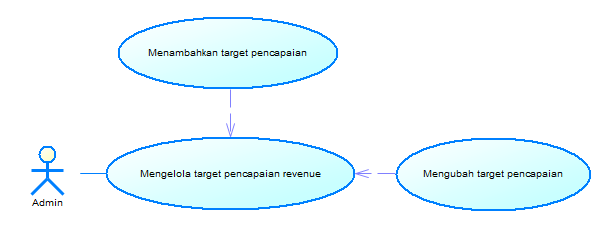
\includegraphics[width=10cm,height=4cm]{bab4/use_case_mengelola_target_pencapaian_revenue.png}}
		\caption{Diagram \textit{Use Case} Mengelola Target Pencapaian \textit{Revenue}}
		\label{figure:use_case_mengelola_target_pencapaian}
	\end{figure}

	\subsubsection{Menambah Target Pencapaian \textit{Revenue}}
	Pengguna dapat menambahkan target pencapaian \textit{revenue} untuk tiap cluster yang ada. Diagram \ref{figure:activity_menambah_target_pencapaian_revenue} adalah diagram aktivitas menambah target pencapaian \textit{revenue} pada sistem TPORT.
	
	\begin{figure}[h]
	\centerline {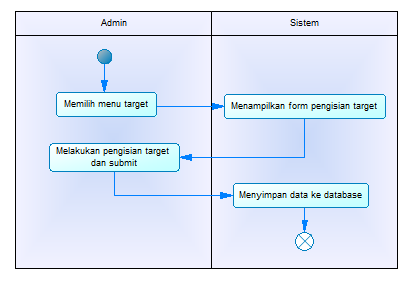
\includegraphics[width=9cm,height=6cm]{bab4/activity_menambah_target_pencapaian_revenue.png}}
	\caption{Diagram Aktivitas Menambah Target Pencapaian \textit{Revenue}}
	\label{figure:activity_menambah_target_pencapaian_revenue}
	\end{figure}
		
	\subsubsection{Mengubah Target Pencapaian \textit{Revenue}}
	User dapat mengubah data target pencapaian yang telah ditambahkan. Diagram \ref{figure:activity_mengubah_target_pencapaian_revenue} adalah diagram aktivitas mengubah target pencapaian \textit{revenue} pada sistem TPORT.
	
	\begin{figure}[h]
	\centerline {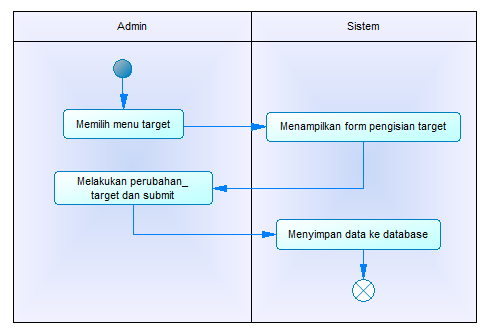
\includegraphics[width=9cm,height=5.6cm]{bab4/activity_mengubah_target_pencapaian_revenue.png}}
	\caption{Diagram Aktivitas Mengubah Target Pencapaian \textit{Revenue}}
	\label{figure:activity_mengubah_target_pencapaian_revenue}
	\end{figure}		
	
\section{Melihat Finish}
Berikut adalah deskripsi dan diagram aktivitas pada \textit{use case} Melihat Finish.
\subsection{Deskripsi Umum Sistem}
\tab Sistem dapat menampilkan daftar permintaan relokasi dengan status telah dibayar.
\subsection{\textit{Use Case} dan Fitur Sistem}
Gambar \ref{figure:use_case_melihat_finish} adalah \textit{use case} melihat daftar permintaan relokasi dengan status telah dibayar. Pada halaman melihat daftar permintaan relokasi dengan status telah dibayar, user dapat melakukan beberapa kegiatan sebagai berikut:
	\subsubsection{Melihat Finish}
	User dapat melihat daftar permintaan relokasi dengan status telah dibayar. Diagram \ref{figure:activity_melihat_finish} adalah diagram aktivitas melihat daftar penagihan pembayaran permintaan relokasi pada sistem \textit{Monitoring} SIK.
	\begin{figure}[h]
	\centerline {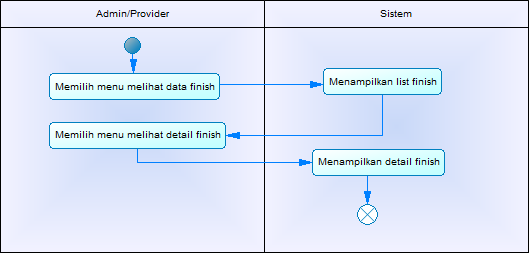
\includegraphics[width=9cm,height=5.5cm]{bab4/ActivityDiagram_MelihatFinish.png}}
	\caption{Diagram Aktivitas Melihat Daftar Permintaan Relokasi Sudah Dibayar}
	\label{figure:activity_melihat_finish}
	\end{figure}

	\begin{figure}[h!]
	\centerline
	{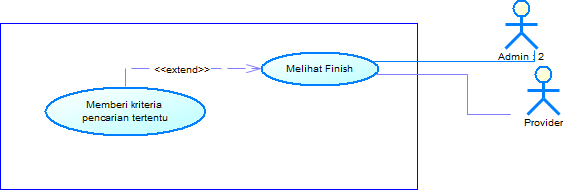
\includegraphics[width=9cm,height=5cm]{bab4/use-case-melihat-finish.png}}
	\caption{Diagram \textit{Use Case} Melihat Daftar Permintaan Relokasi Sudah Dibayar}
	\label{figure:use_case_melihat_finish}
	\end{figure}
	
\newpage
\section{Perancangan Data}
\tab Dalam pembuatan sebuah sistem informasi, database merupakan salah satu faktor utama yang penting. Perancangan dan alur data pada sebuah sistem harus dapat memenuhi kebutuhan-kebutuhan sistem, meliputi penambahan data, perubahan isi data dan penghapusan data dari basisdata sistem. Berikut adalah perancangan data pada sistem informasi \textit{monitoring} SIK.
\subsection{\textit{Conceptual Data Model}}
CDM (\textit{Conceptual Data Model}) merupakan sebuah model yang didasarkan pada objek-objek di dunia nyata. Objek dasar tersebut direpresentasikan dalam bentuk \textit{entity relationship diagram}. Gambar \ref{figure:CDM} adalah CDM pada pembuatan sistem informasi \textit{monitoring} SIK.
	\begin{figure}[h!]
	\centerline
	{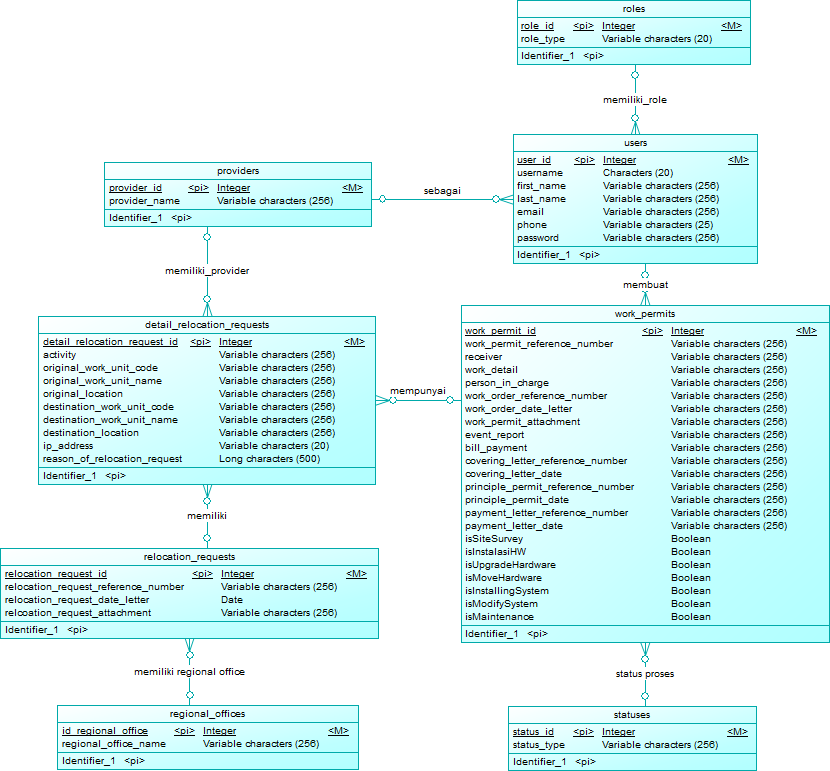
\includegraphics[width=10cm,height=14cm]{bab4/CDM.png}}
	\caption{Diagram \textit{Conceptual Data Model}}
	\label{figure:CDM}
	\end{figure}
	
\subsection{\textit{Physical Data Model}}
PDM (\textit{Physical Data Model}) adalah model yang digambarkan dalam sebuah tabel serta hubungan-hubungan antara data dengan tabel lain. Gambar \ref{figure:PDM} adalah PDM pada pembuatan sistem informasi \textit{monitoring} SIK.
	\begin{figure}[h!]
	\centerline
	{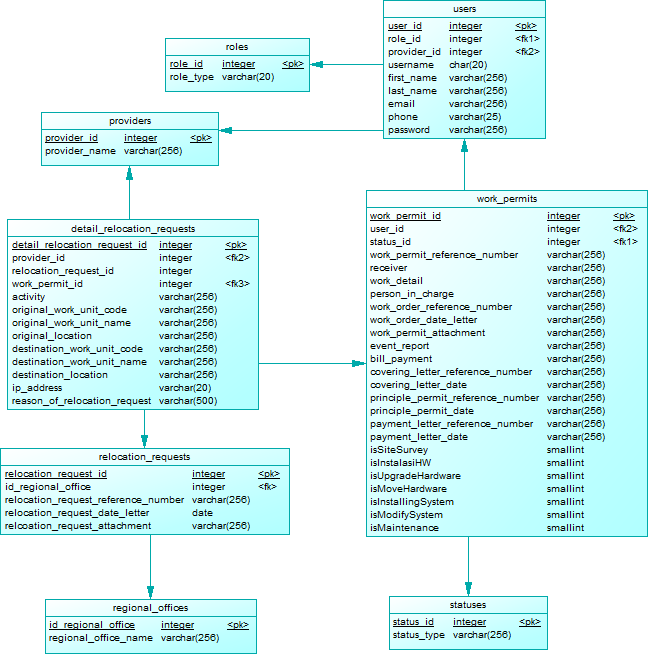
\includegraphics[width=10cm,height=11cm]{bab4/PDM.png}}
	\caption{Diagram \textit{Physical Data Model}}
	\label{figure:PDM}
	\end{figure}